\begin{enumerate}
    \item \textbf{Axit amin trong protein.} \\
    Mật độ năng lượng điện trường trong môi trường $\epsilon$ bất kỳ:
\begin{equation} \label{eq1_Protein}
    \omega = \dfrac{1}{2}\epsilon\epsilon_0E^2 = \dfrac{kq^2}{8\pi\epsilon k  r^4}.
\end{equation}
Năng lượng tĩnh điện trong môi trường $\epsilon$ bất kỳ:
\begin{equation} \label{eq2_Protein}
    W =\displaystyle\int\limits^{\infty}_{R}\omega 4\pi r^2dr=\displaystyle\int\limits^{\infty}_{R}\dfrac{kq^2}{2\epsilon r^2}dr  =\dfrac{kq^2}{2\epsilon R}.
\end{equation}
Thay số:
\begin{align} 
    \label{eq3_Protein}
    W_p&\approx 2.56 \times 10^{-19} \ \si{J} \approx 36.86 \ \si{kcal/mol},\\
    \label{eq4_Protein}
    W_w&\approx 9.61 \times 10^{-21} \ \si{J} \approx 1.38 \ \si{kcal/mol}.
\end{align}
Độ chênh lệch năng lượng:
\begin{equation} \label{eq5_Protein}
    \Delta W = |W_w - W_p| = 35.48 \ \si{kcal/mol}.
\end{equation}
Như vậy độ chênh năng lượng tĩnh điện khi điện tích đi từ nước vào protein hay chính bằng năng lượng cung cấp cho cấu trúc protein sẽ rất lớn so với năng lượng cần để phá huỷ cấu trúc protein, vì vậy bên trong protein hầu như axit amin không tích điện để không phá huỷ cấu trúc protein. \\
\textit{Trên thực tế, vẫn có các cấu trúc phân tử tích điện xuất hiện bên trong protein nhưng các phân tử này đóng vai trò của các nhóm chức năng và tham gia các hoạt động sinh học của protein chứ không phải nhóm cấu tạo nên không làm phá huỷ cấu trúc protein.}
     \item \textbf{Tương tác giữa điện tích và protein trong môi trường nước.}
     \begin{enumerate}[label=\textbf{\alph*,}]\itemsep0em
         \item Ta sử dụng phương pháp ảnh điện. Giả sử ban đầu điện tích $q$ có toạ độ $\Vec{r}_0$ ($R\ll|\Vec{r}_0| \ll |\Vec{r}|$) với gốc là một điểm nằm trên mặt phân cách $(A)$ \textbf{(Hình 3)}. Để thoả mãn điều kiện biên của điện trường tại mọi điểm trên mặt phân cách $(A)$, hệ tương đương như sau:
         \begin{enumerate}
             \item Điện tích ảnh $q'=\dfrac{\epsilon_w-\epsilon_p}{\epsilon_w+\epsilon_p}q$ của điện tích $q$ qua mặt $(A)$, trong môi trường nước, đặt tại $\Vec{r}_1=-\Vec{r}_0$.
             \item Điện tích ảnh $q''=\dfrac{2\epsilon_p}{\epsilon_w+\epsilon_p}q$ của điện tích $q'$ qua mặt $(A)$, trong môi trường protein, đặt tại $\Vec{r}_2=\Vec{r}_0$.
         \end{enumerate}
\begin{center}
    \begin{figure}[htp]
    \begin{center}
        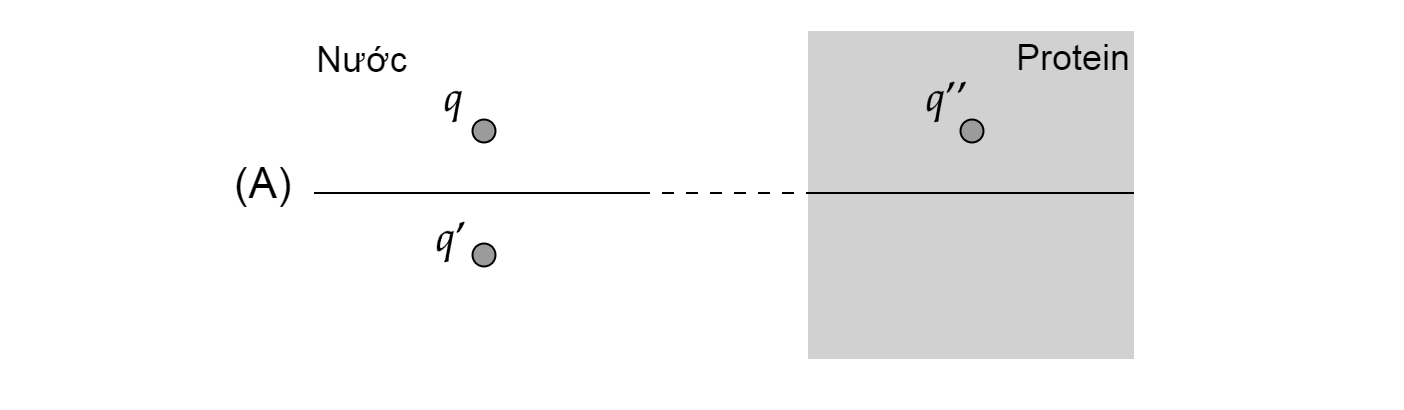
\includegraphics[scale=.27
        ]{Problem_13/image/3.png}
    \end{center}
    \begin{center}
    Hình 3: Điện tích $q$ và các điện tích ảnh tương ứng.
    \end{center}
    \end{figure}
\end{center}
         Điện tích $q$ và $q'$ tham gia vào tương tác tĩnh điện trong vùng môi trường nước chứa điện tích, $q''$ tham gia vào vùng môi trường protein. Thế năng tĩnh điện trong từng vùng môi trường:
\begin{align}
    \label{eq6_Protein}
    V_{\text{nước}\uparrow}&=\dfrac{kq}{\epsilon_w \left|\Vec{r}-\Vec{r}_0\right|}+\dfrac{kq'}{\epsilon_w \left|\Vec{r}-\Vec{r}_1\right|} \approx \dfrac{k(q+q')}{\epsilon_w r}=\dfrac{2kq}{(\epsilon_w+\epsilon_p) r}, \\
    \label{eq7_Protein}
    V_{\text{protein}}&=\dfrac{kq''}{\epsilon_p \left|\Vec{r}-\Vec{r}_2\right|} \approx \dfrac{kq''}{\epsilon_p r}=\dfrac{2kq}{(\epsilon_w+\epsilon_p) r}.
\end{align}
Từ phương trình (\ref{eq6_Protein}) ta suy ra hằng số điện môi hiệu dụng tương ứng với vùng môi trường nước chứa điện tích:
\begin{equation} \label{eq8_Protein}
    \epsilon_{\text{eff}}^{(1)}=\dfrac{\epsilon_w+\epsilon_p}{2}=41.50.
\end{equation}
          \item  Từ phương trình (\ref{eq7_Protein}) ta suy ra hằng số điện môi hiệu dụng tương ứng với vùng môi trường bên trong protein:
\begin{equation} \label{eq9_Protein}
    \epsilon_{\text{eff}}^{(2)}=\dfrac{\epsilon_w+\epsilon_p}{2}=41.50.
\end{equation}
          \item Do khi khảo sát tĩnh điện ở vùng không gian môi trường nước không chứa điện tích, các lưỡng cực trong nước bị phân cực mạnh hơn trong protein nên ta chỉ xét ảnh hưởng của các điện tích liên kết trong môi trường nước ở mặt phân cách xa điện tích $q$ nên điện tích tham gia vào tương tác chỉ có điện tích ảnh sinh ra do các điện tích liên kết trong môi trường nước hình thành ở mặt phân cách xa điện tích $q$. Điện tích này tương tự điện tích ảnh $q''$ đối với chính $q''$, ta gọi là $q'''$ \textbf{(Hình 4)}. Điện tích ảnh $q'''=\dfrac{2\epsilon_w}{\epsilon_p+\epsilon_w}q''=\dfrac{4\epsilon_w\epsilon_p}{(\epsilon_w+\epsilon_p)^2}q$ của điện tích $q''$ qua mặt $(B)$, trong môi trường nước, đặt tại $\Vec{r}_3$.\\
\begin{center}
    \begin{figure}[htp]
    \begin{center}
        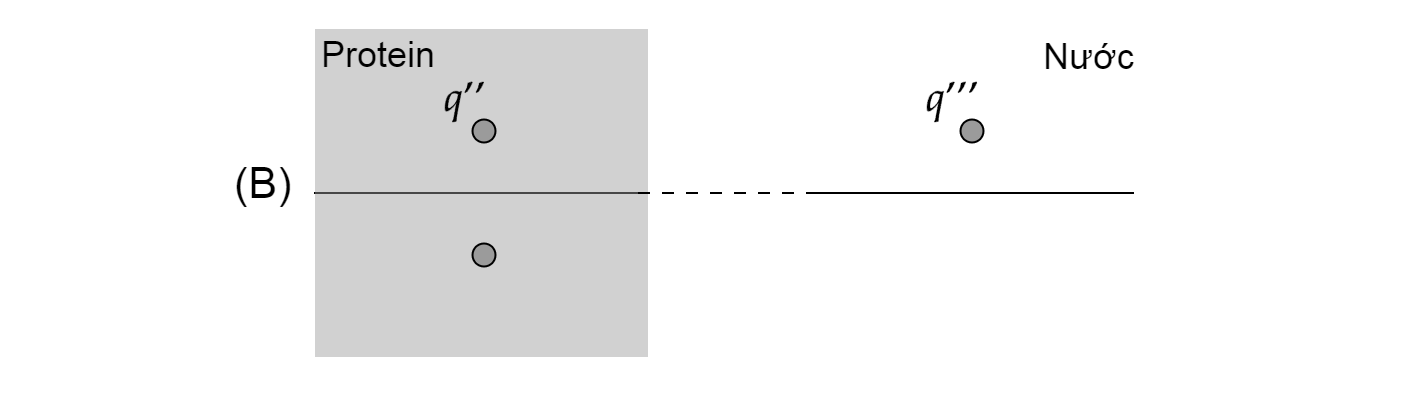
\includegraphics[scale=.27
        ]{Problem_13/image/4.png}
    \end{center}
    \begin{center}
    Hình 4: Điện tích $q''$ và điện tích ảnh $q'''$.
    \end{center}
    \end{figure}
\end{center}
          Thế năng tĩnh điện trong vùng môi trường nước không chứa điện tích:
          \begin{equation} \label{eq10_Protein}
              V_{\text{nước}\downarrow}=\dfrac{kq'''}{\epsilon_w \left|\Vec{r}-\Vec{r}_3\right|} \approx \dfrac{kq'''}{\epsilon_w r}=\dfrac{4\epsilon_p kq}{(\epsilon_w+\epsilon_p)^2 r}.
          \end{equation}
          Từ phương trình (\ref{eq10_Protein}) ta suy ra hằng số điện môi hiệu dụng tương ứng với vùng môi trường nước không chứa điện tích:
          \begin{equation} \label{eq11_Protein}
          \epsilon_{\text{eff}}^{(3)}=\dfrac{(\epsilon_w+\epsilon_p)^2}{4\epsilon_p}\approx 574.08.
          \end{equation}
     \end{enumerate}
     \textit{Kết quả thực nghiệm cho kết quả (11) chỉ cỡ 200, giải thích cho điều này là do kích thước của protein hữu hạn nên gần đúng chúng ta sử dụng trong bài tương đối cực đoan, nhưng dù sao 200 vẫn là con số khá lớn so với 41,5. Các thí nghiệm bởi nhóm nghiên cứu của Alan Fersht cho thấy những ước tính trên cũng phù hợp với protein. Trong các thí nghiệm của Fersht, các đột biến được thực hiện trên bề mặt của protein để không làm hỏng cấu trúc của nó. Kết quả thực nghiệm cho thấy: hằng số điện môi hiệu dụng nằm trong khoảng từ 40 đến 200. Thực tế là $\epsilon_{\text{eff}}$ có thể đạt đến giá trị 200 không có gì đáng ngạc nhiên sau các xem xét chúng ta đã thực hiện ở trên. Phương pháp ảnh điện phổ thông đã mô tả và giải thích khá thành công cho một số hiện tượng vật lý trong sinh học (Bạn có thể tham khảo một số công trình khoa học của GS. TS Nguyễn Thế Toàn về vật lý sinh).}
     \item \textbf{Tương tác giữa điện tích và protein trong môi trường có ion tự do.} \\ 
     Phương trình Poisson:
\begin{equation} \label{eq12_Protein}
    \nabla^2_r V(r) = - \dfrac{4\pi k \rho}{\epsilon_{\text{eff}}} = - \dfrac{4\pi k \text{e}}{\epsilon_{\text{eff}}}\sum\limits_i {{c_i}{N_i}} {e^{ - E_i/k_BT}} \approx - \dfrac{4\pi k \text{e}}{\epsilon_{\text{eff}}}\sum\limits_i {{c_i}{N_i}}\left(1- \dfrac{E_i}{k_BT}\right).
\end{equation}
Năng lượng của ion loại $i$:
\begin{equation} \label{eq13_Protein}
    E_i=\text{e}N_iV(r).
\end{equation}
Thay phương trình (\ref{eq13_Protein}) vào phương trình (\ref{eq12_Protein}):
\begin{equation} \label{eq14_Protein}
    \nabla^2_r V(r) =  \dfrac{4\pi k \text{e}}{\epsilon_{\text{eff}}}\sum\limits_i {{c_i}{N_i}} \left(\dfrac{\text{e}N_iV(r)}{k_BT}-1 \right)=\dfrac{8\pi k \text{e}^2 V(r)}{\epsilon_{\text{eff}}k_BT}\sum\limits_i \dfrac{1}{2}{{c_i}{N_i^2}} - \dfrac{4\pi k \text{e}}{\epsilon_{\text{eff}}}\sum\limits_i {{c_i}{N_i}}.
\end{equation}
Do hệ ion trung hoà nên $\sum\limits_i {{c_i}{\text{e}N_i}}=0$, phương trình (\ref{eq14_Protein}) trở thành:
\begin{equation} \label{eq15_Protein}
    \nabla^2_r V(r)=\dfrac{8\pi k \text{e}^2 V(r)}{\epsilon_{\text{eff}}k_BT}I.
\end{equation}
Mặt khác, theo đề bài, $V(r)=\dfrac{kq}{\epsilon_{\text{eff}}}\dfrac{e^{-r/D}}{r}$, thay vào vế trái phương trình (\ref{eq15_Protein}) ta được:
\begin{equation} \label{eq16_Protein}
    \nabla^2_r V(r)=\dfrac{1}{D^2} V(r).
\end{equation}
Từ phương trình (\ref{eq15_Protein}) và phương trình (\ref{eq16_Protein}) ta suy ra:
\begin{equation} \label{eq17_Protein}
    \dfrac{1}{D^2}=\dfrac{8\pi k \text{e}^2 I}{\epsilon_{\text{eff}}k_BT} \Rightarrow 
    D= \sqrt{\dfrac{\epsilon_{\text{eff}}k_BT}{8\pi k \text{e}^2 I}}.
\end{equation}
Thay số: $D\approx 6.21\times 10^{-10}\ \si{m} = 6.21\ \si{\angstrom}$.\\
\textit{Qua bài tập này, ta thấy được một tính chất rất quan trọng trong nghiên cứu về tế bào, đó là tương tác tĩnh điện không chỉ phụ thuộc vào khoảng cách và điện tích, mà còn phụ thuộc cả đặc tính của môi trường như nhiệt độ, nồng độ ion, thậm chí còn phụ thuộc cả vào hình dạng của vật thể tương tác do hằng số điện môi hiệu dụng phụ thuộc vào hình dạng của vật.}
\end{enumerate}

\textbf{Biểu điểm}
\begin{center}
\begin{tabular}{|>{\centering\arraybackslash}m{1cm}|>{\raggedright\arraybackslash}m{14cm}| >{\centering\arraybackslash}m{1cm}|}
    \hline
    \textbf{Phần} & \textbf{Nội dung} & \textbf{Điểm} \\
    \hline
    \textbf{1} & Viết biểu thức năng lượng tĩnh điện trong môi trường $\epsilon$ (\ref{eq2_Protein}) & $0.50$ \\
    \cline{2-3}
    &  Tính được độ chênh lệch năng lượng giữa môi trường nước và môi trường protein (\ref{eq5_Protein}) & $0.50$ \\
    \cline{2-3}
    &  Lập luận và kết luận & $0.50$ \\
    \hline
    \textbf{2a} & Chỉ ra điện tích ảnh $q'$ & $0.50$ \\
    \cline{2-3}
     & Chỉ ra điện tích ảnh $q''$ & $0.50$ \\
    \cline{2-3}
    & Viết biểu thức năng lượng tĩnh điện trong vùng môi trường nước chứa điện tích $q$ (\ref{eq6_Protein}) & $0.50$ \\
    \cline{2-3}
    & Viết biểu thức năng lượng tĩnh điện trong vùng môi trường protein $q$ (\ref{eq7_Protein}) & $0.50$ \\
    \cline{2-3}
    & Tính được hằng số điện môi $\epsilon_{\text{eff}}^{(1)}$ (\ref{eq8_Protein}) & $0.50$ \\
    \hline
    \textbf{2b} & Tính được hằng số điện môi $\epsilon_{\text{eff}}^{(2)}$ (\ref{eq9_Protein}) & $0.50$ \\
    \hline
    \textbf{2c} & Chỉ ra điện tích ảnh $q'''$ & $0.50$ \\
    \cline{2-3}
    & Viết biểu thức năng lượng tĩnh điện trong vùng môi trường nước chứa điện tích $q$ (\ref{eq10_Protein}) & $0.50$ \\
    \cline{2-3}
    & Tính được hằng số điện môi $\epsilon_{\text{eff}}^{(3)}$ (\ref{eq11_Protein}) & $0.50$ \\
    \hline
    \textbf{3} & Dẫn ra phương trình Poisson (\ref{eq12_Protein}) & $0.50$ \\
    \cline{2-3}
    & Gần đúng phương trình Poisson và thu được phương trình (\ref{eq15_Protein}) & $0.50$ \\
    \cline{2-3}
    & Dẫn ra phương trình (\ref{eq16_Protein}) & $0.50$ \\
    \cline{2-3}
    & Viết biểu thức cho bán kính chắn Debye-Huckel và thay số (\ref{eq17_Protein}) & $0.50$ \\
    \hline
\end{tabular}
\end{center}

%% Reference %%
\bibliographystyle{plain}
\begin{thebibliography}{}
\bibitem{ttn2000} T. T. Nguyen, A. Yu. Grosberg, B. I. Shklovskii (2000), \textit{Macroions in Salty Water with Multivalent Ions: Giant Inversion of Charge}, Physical Review Letters, Volume 85, Issue 7, Pages 1568-1571.
\bibitem{fersht1989} Alan R. Fersht, Michael J. E. Sternberg (1989), \textit{Can a simple function for the dielectric response model electrostatic effects in globular proteins?}, Protein Engineering, vol.2 no.15 pp.527-530.
\bibitem{ladau1980} L. D. Landau, E. M. Lifshitz (1980), \textit{Statical Physics}.
\bibitem{finkelstein1964} Alexi V. Finkelstein, Oleg Ptitsyn (1964), \textit{Protein Physics: A course of lectures}.
\bibitem{Toan2021} Nguyễn Thế Toàn, Nguyễn Hoạ Mi (2021), \textit{Giáo trình Vật lý Sinh học của Protein}, NXB ĐHQGHN.
\bibitem{brooks1987} Charles L. Brooks III, Martin Karplus, B. Montgomery Pettitt (1987), \textit{Proteins: A Theoretical Perspective of Dynamics, Structure, and Thermodynamics}.
\end{thebibliography}